% vim: ai sw=2

\documentclass[xcolor=dvipsnames]{beamer}

\let\Oldemph\emph
\renewcommand{\emph}[1]{\textcolor{blue}{\Oldemph{#1}}}
\newcommand{\heading}[1]{\textbf{\textcolor{BurntOrange}{#1}}}
\newcommand{\header}[1]{\textbf{\texttt{\textcolor{WildStrawberry}{#1}}}}
\newcommand{\doc}[1]{\textbf{\texttt{\textcolor{OliveGreen}{#1}}}}

% Copyright 2004 by Till Tantau <tantau@users.sourceforge.net>.
%
% In principle, this file can be redistributed and/or modified under
% the terms of the GNU Public License, version 2.
%
% However, this file is supposed to be a template to be modified
% for your own needs. For this reason, if you use this file as a
% template and not specifically distribute it as part of a another
% package/program, I grant the extra permission to freely copy and
% modify this file as you see fit and even to delete this copyright
% notice.


\mode<presentation>
{
%  \usetheme{Warsaw}
\usetheme{Madrid}

  \setbeamercovered{transparent}
}

\usepackage[czech]{babel}
\usepackage[utf8]{inputenc}
\usepackage{times}
\usepackage[IL2]{fontenc}

\usepackage{graphicx}
\usepackage[final]{listings}
\usepackage{multirow}

\lstset{tabsize=2,numbers=none,showstringspaces=false,breaklines=true,
	breakatwhitespace=true,escapeinside={(*@}{@*)},
	basicstyle=\scriptsize,keywordstyle=\bfseries\color{OliveGreen},
	commentstyle=\color{blue}}

\title[Libe-router] % (optional, use only with long paper titles)
{Where is the (Libe)router}

%\subtitle{X.}

\author[J. Slabý]{Jiří~Slabý}

\institute[Liberouter] % (optional, but mostly needed)
{Liberouter, Brno}

\date{3. 12. 2010}

\subject{}
% This is only inserted into the PDF information catalog. Can be left
% out.



% If you have a file called "university-logo-filename.xxx", where xxx
% is a graphic format that can be processed by latex or pdflatex,
% resp., then you can add a logo as follows:

% \pgfdeclareimage[height=0.5cm]{university-logo}{university-logo-filename}
% \logo{\pgfuseimage{university-logo}}



% Delete this, if you do not want the table of contents to pop up at
% the beginning of each subsection:
% \AtBeginSubsection[]
% {
%   \begin{frame}<beamer>
%     \frametitle{Outline}
%     \tableofcontents[currentsection,currentsubsection]
%   \end{frame}
% }


% If you wish to uncover everything in a step-wise fashion, uncomment
% the following command:

%\beamerdefaultoverlayspecification{<+->}

\begin{document}

\begin{frame}
  \titlepage
\end{frame}

%%%%%%%%%%%%%%%%%%%%%%%

\begin{frame}
  \frametitle{Struktura prezentace}

  \begin{enumerate}
  \item Kde je doopravdy Libe-router
  \begin{itemize}
  \item Velmi malý výlet do historie
  \end{itemize}
  \item \emph{Vranovskoveský zázrak}
  \end{enumerate}

\end{frame}

\begin{frame}
  \frametitle{Liberouter}

  \heading{Co je to Liberouter?}
  \begin{quote}
The aim of the Liberouter project is the development of a dual-stack (IPv6 and
IPv4) gigabit router based on the standard PC architecture with a
high-performance hardware accelerator of packet forwarding and filtering. This
way we can improve the throughput of a PC router platform compared to the
software-only solution.
  \end{quote}

  \pause

  \begin{center}
  \heading{Ale kde tedy je?}
  \end{center}

\end{frame}

\begin{frame}
  \frametitle{Liberouter}

  \begin{itemize}
  \item Myšlenka se časem vytratila\ldots
  \pause
  \item \ldots aby byla znovu objevena
  \begin{itemize}
  \item Vedení dalo hlavy dohromady
  \item Vymýšlely, jak (stylově) zakončit projekt MSM6383917201
  \end{itemize}
  \end{itemize}

\end{frame}

\begin{frame}
  \frametitle{Co máme?}

  \begin{itemize}
  \item Superrychlé karty (ComboV2)
  \item 4 porty po 10Gbit (NIC)
  \item Rozdělení zátěže (HANIC)
  \end{itemize}

  \pause
  \bigskip

  \begin{center}
  \heading{Otázka: a proč z toho neudělat rychlý router?} \\
  \heading{Odpověď z Vranovské Vsi: no proč ne\ldots}
  \end{center}

\end{frame}

\begin{frame}
  \frametitle{Vranovskoveský zázrak}

  \heading{Postup -- 3 fáze}
  \begin{enumerate}
  \item Procedit všechnu zátěž přes IP stack (zdarma)
  \item Odlehčit IP stacku a něco směrovat v SW ještě před stackem
  \item Odlehčit SW a něco směrovat už v HW
  \end{enumerate}

\end{frame}

\begin{frame}
  \frametitle{IP stack směrování}

  \heading{1. fáze}
  \begin{itemize}
  \item Všechna data směruje IP stack
  \item Dvojí kopírování
  \begin{itemize}
  \item Z kruhového bufferu do socket bufferu
  \item Ze socket bufferu do jiného kruhového bufferu
  \end{itemize}
  \item Vysoká zátěž CPU
  \item \emph{Stav}: hotovo
  \begin{itemize}
  \item Není co programovat
  \end{itemize}
  \end{itemize}

\end{frame}

\begin{frame}
  \frametitle{IP stack směrování}

  \begin{figure}
  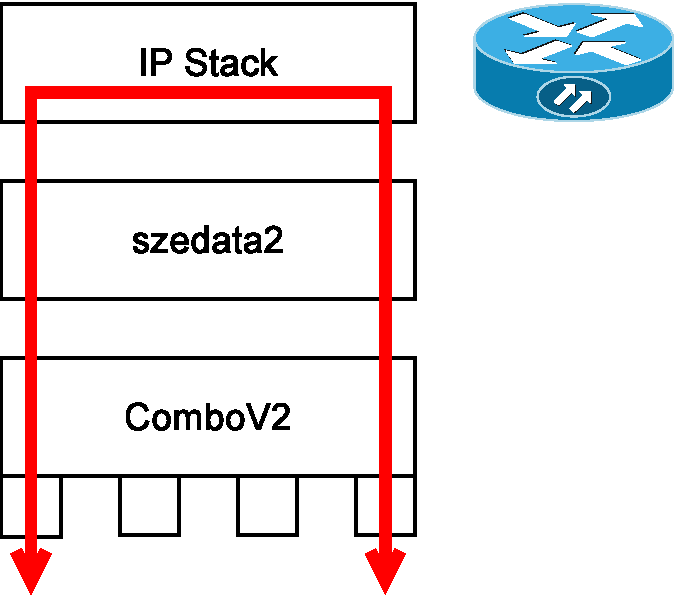
\includegraphics[height=170px]{router-IP}
  \caption{Fáze 1}
  \end{figure}

\end{frame}

\begin{frame}
  \frametitle{Szedata2 směrování}

  \heading{2. fáze}
  \begin{itemize}
  \item Většinu dat směruje sze2
  \begin{itemize}
  \item Podle směrovací tabulky jádra
  \end{itemize}
  \item Zbytek dat zpracovává IP stack
  \begin{itemize}
  \item Např. ARP provoz
  \end{itemize}
  \item Jedno kopírování
  \begin{itemize}
  \item Z jednoho kruhového bufferu do druhého
  \end{itemize}
  \item Vysoká zátěž CPU
  \item \emph{Stav}: v řešení
  \begin{itemize}
  \item Je třeba jednoduchý parser a zavolání směrovací funkce
  \end{itemize}
  \end{itemize}

\end{frame}

\begin{frame}
  \frametitle{Szedata2 směrování}

  \begin{figure}
  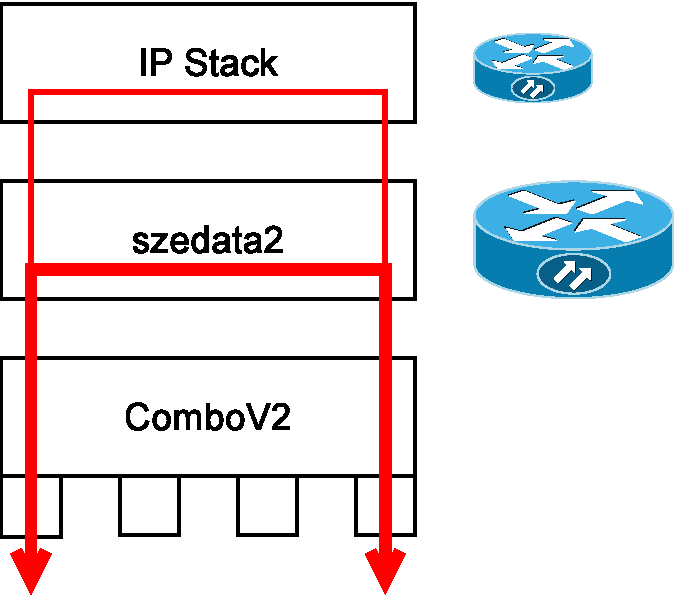
\includegraphics[height=170px]{router-sze}
  \caption{Fáze 2}
  \end{figure}

\end{frame}

\begin{frame}
  \frametitle{HW směrování}

  \heading{3. fáze}
  \begin{itemize}
  \item Většinu dat směruje HW
  \begin{itemize}
  \item Podle uložené směrovací tabulky
  \end{itemize}
  \item Zbytek dat zpracovává sze2 a IP stack
  \item Žádné kopírování
  \begin{itemize}
  \item Data jsou směrována přímo v HW
  \end{itemize}
  \item Nízká zátěž CPU
  \item \emph{Stav}: v návrhu
  \end{itemize}

\end{frame}

\begin{frame}
  \frametitle{HW směrování}

  \begin{figure}
  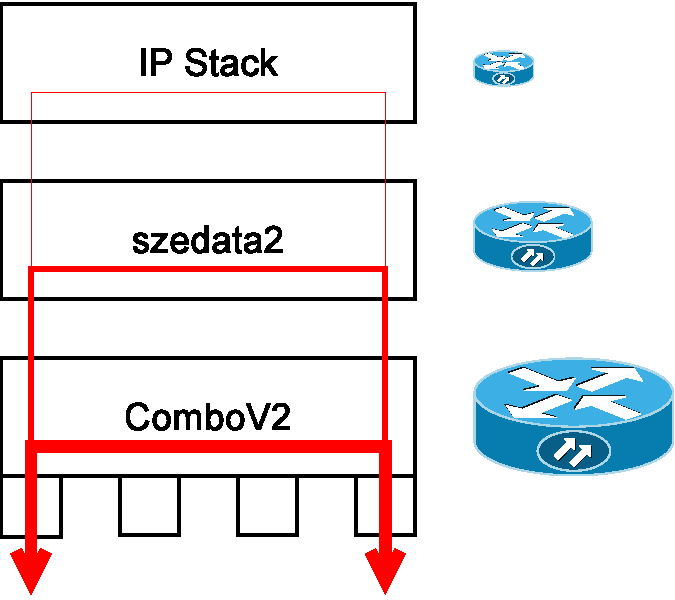
\includegraphics[height=170px]{router-HW}
  \caption{Fáze 3}
  \end{figure}

\end{frame}

\begin{frame}
  \frametitle{Závěr}

  \begin{itemize}
  \item Libe-router reloaded
  \item Slibné zakončení projektu Ministerstva
  \end{itemize}

\end{frame}

\begin{frame}
  \frametitle{Konec}

  \begin{center}
  \huge
  \heading{Děkuji za pozornost}\\[1em]
  \heading{Dotazy?}
  \end{center}

\end{frame}

\end{document}

